\chapter{Конструкторский раздел}
В данном разделе приведено описание решения всех конструкторских задач.

\section{Конечный автомат состояний сервера}

На рис.~\ref{fig:fsm} приведен конечный автомат, описывающий состояния SMTP-сервера. 

Состояния автомата:

\begin{enumerate}
\item \textbf{START} ~-- начальное состояние автомата
\item \textbf{INITIALIZED} ~--  клиенту отправлена строка приветствия, состояние готовности приема команд, все буферы очищены
\item \textbf{MAIL\_FROM\_ENTERED} ~-- от клиента получена информация об отправителе почты
\item \textbf{RCPT\_TO\_ENTERED} ~-- от клиента получена информация о получателе почты
\item \textbf{DATA\_ENTERED} ~-- состояние ожидания содержимого письма
\item \textbf{POINT\_ENTERED} ~-- от клиента получена команда завершения передачи содержимого письма
\item \textbf{END} ~-- завершающее состояние, получена команда \textbf{QUIT} или произошел таймаут
\end{enumerate}



\begin{figure}
\centering
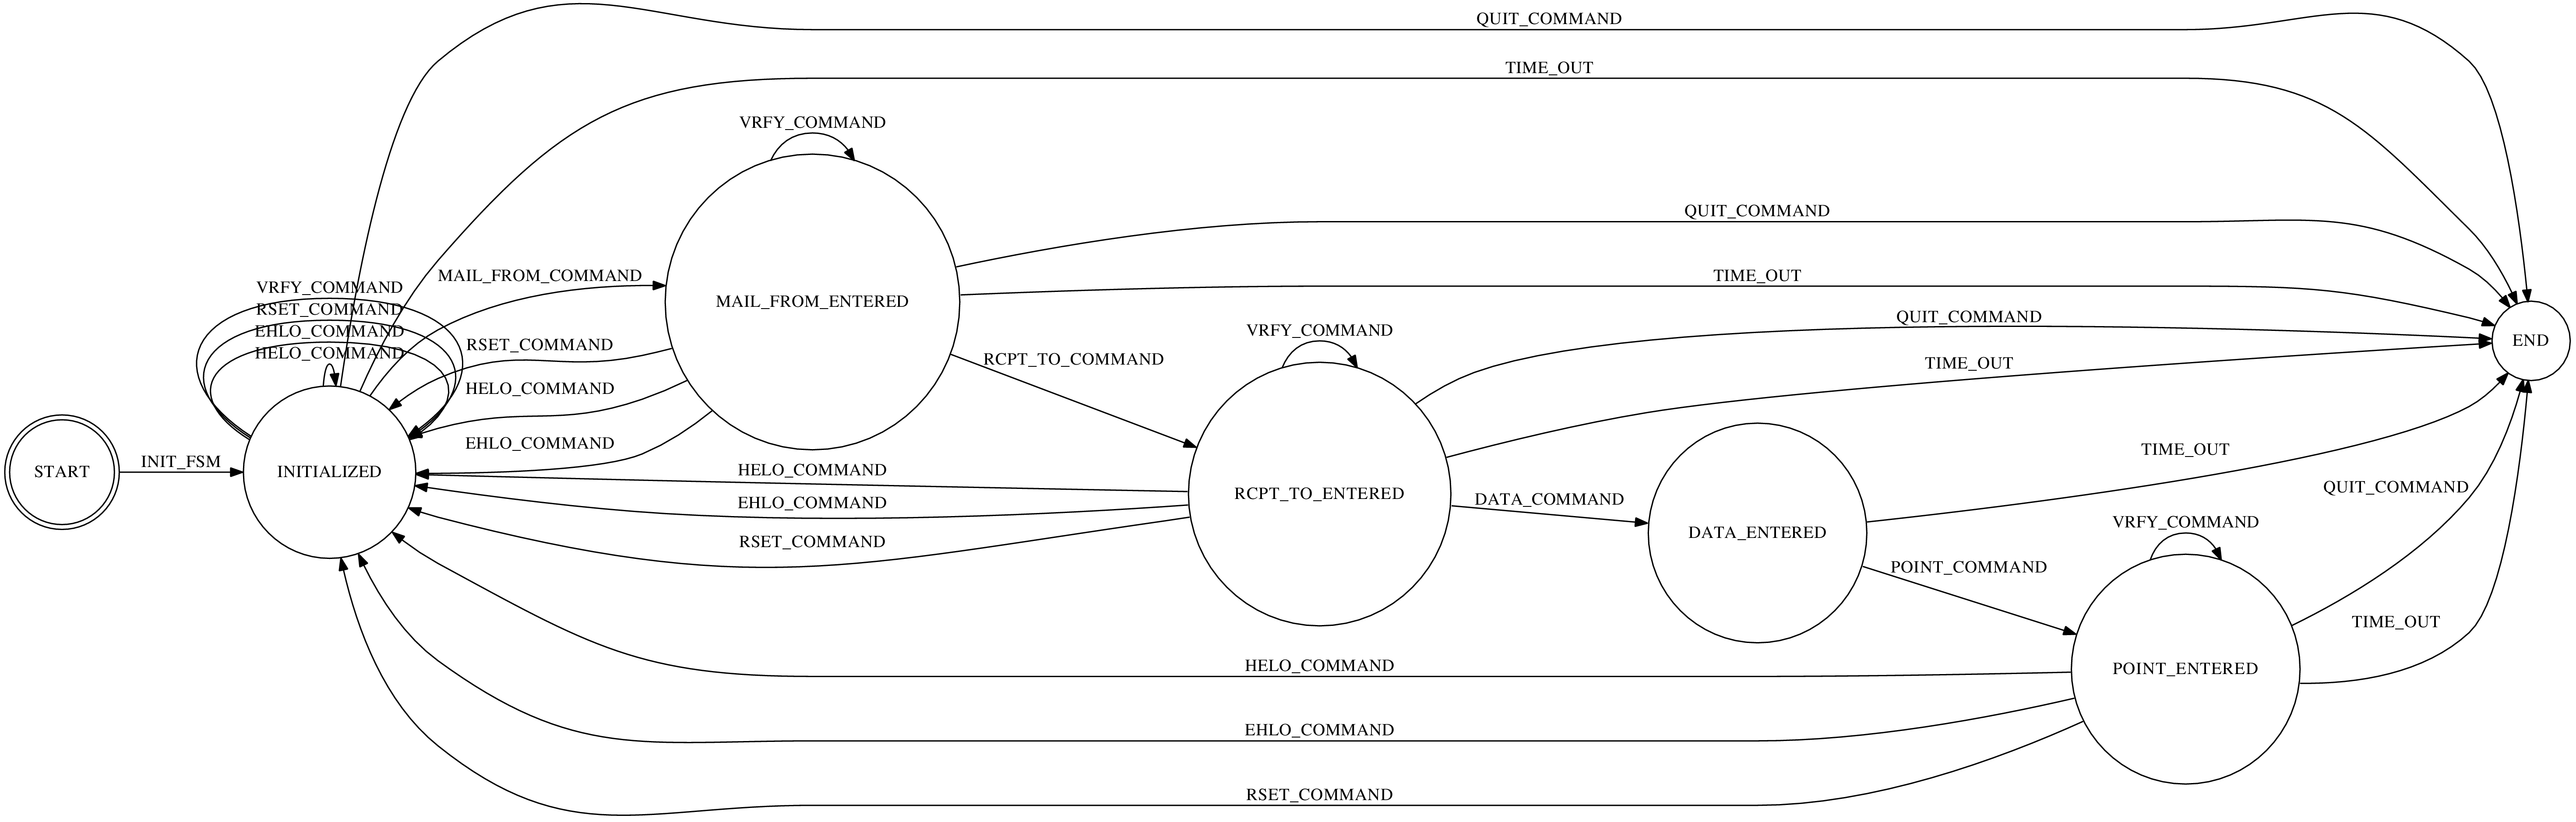
\includegraphics[angle=90,width=0.6\textwidth]{smtp.png}
\caption{Состояния сервера}
\label{fig:fsm}
\end{figure}


\section{Проектирование алгоритмов обработки соединений}

Сервер состоит из следующих процессов: основной процесс сервера, несколько рабочих процессов.

\subsection{Логика работы основного процесса}
Основной процесс системы инициализирует необходимые структуры данных, создает сокет для прослушивания и запускает остальные процессы. В листинге~\ref{lst:pseudomain} приведен псевдокод, описывающий логику работы основного процесса сервера.

\begin{lstlisting}[caption={Логика работы основного процесса},label=lst:pseudomain]
int main()
{
    int result = read_config_file();
    if (result)
        return (EXIT_FAILURE);

    result = mkdir_if_not_exists(mail_dir_path);
    if (result)
        fprintf(stderr, "mkdir_if_not_exists failed: %s\n", mail_dir_path);

    Logger logger = Logger_create(log_file_name);
    log_info(logger, "Server started\n");

    char buffer[1024];
    char buffer_temp[1024];
    int rc;
    int len;
    int new_sd = -1;
    int end_server = 0, compress_array = 0;
    int close_conn;
    int timeout;
    int listen_sd = create_socket();
    int nfds = 1, current_size = 0, i, j;
    
    struct contexts head;              
    
    LIST_INIT(&head.list);             
    
    int fork_index;
    for (fork_index = 0; fork_index < workers_count; ++fork_index){
        int pid = fork();
        switch(pid) {
        case -1:
            perror("fork");
            return 1;
        case 0:{
            struct pollfd fds[200];
            /*Initialize the pollfd structure*/
            memset(fds, 0 , sizeof(fds));

            /*Set up the initial listening socket*/
            fds[0].fd = listen_sd;
            fds[0].events = POLLIN;

            /*Initialize the timeout to 3 minutes. If no
            activity after 3 minutes this program will end
            timeout value is based on milliseconds*/
            timeout = (3 * 60 * 1000);
            srand(getpid());
            /*Loop waiting for incoming connects or for incoming data
            on any of the connected sockets*/
            do{
                /*Call poll() and wait 3 minutes for it to complete.*/
                printf("Waiting on poll()...\n");
                rc = poll(fds, nfds, timeout);
                ...
            } while (end_server == FALSE); /* End of serving running.*/

            /* Clean up all of the sockets that are open*/
            for (i = 0; i < nfds; i++){
                if(fds[i].fd >= 0)
                    close(fds[i].fd);
            }
        }

        default:
            continue;
        }
    }

    while(1);
    return 0;
}
\end{lstlisting}


\subsection{Логика работы рабочего процесса}
Рабочий процесс получает дескриптор сокета для прослушивания и запускает цикл обслуживания.
В листинге~\ref{lst:pseudoworker} приведен псевдокод, описывающий логику работы рабочего процесса.

\begin{lstlisting}[caption={Логика работы рабочего процесса},label=lst:pseudoworker]
do{
                /*Call poll() and wait 3 minutes for it to complete.*/
                printf("Waiting on poll()...\n");
                rc = poll(fds, nfds, timeout);
                /*Check to see if the poll call failed.*/
                if (rc < 0){
                    perror("  poll() failed");
                    break;
                }

                /*Check to see if the 3 minute time out expired.*/
                if (rc == 0){
                    printf("  poll() timed out.  End program.\n");
                    break;
                }

                /*One or more descriptors are readable.  Need to
                determine which ones they are.*/
                current_size = nfds;
                for (i = 0; i < current_size; i++){
                    /*Loop through to find the descriptors that returned
                    POLLIN and determine whether it's the listening
                    or the active connection.*/
                    if(fds[i].revents == 0)
                        continue;

                    /*If revents is not POLLIN, it's an unexpected result,
                    log and end the server.*/
                    if(fds[i].revents != POLLIN){
                        printf("  Error! revents = %d\n", fds[i].revents);
                        end_server = TRUE;
                        break;
                    }

                    if (fds[i].fd == listen_sd){
                        /*Listening descriptor is readable.*/
                        printf("  Listening socket is readable\n");

                        /*Accept all incoming connections that are
                        queued up on the listening socket before we
                        loop back and call poll again.*/
                        do{
                            /*Accept each incoming connection. If
                            accept fails with EWOULDBLOCK, then we
                            have accepted all of them. Any other
                            failure on accept will cause us to end the
                            server.*/
                            new_sd = accept(listen_sd, NULL, NULL);
                            ...
                            
                            /*Loop back up and accept another incoming
                            connection*/
                        } while (new_sd != -1);
                    }

                    /* This is not the listening socket, therefore an
                    existing connection must be readable*/

                    else{
                        printf("  Descriptor %d is readable\n", fds[i].fd);
                        close_conn = FALSE;

                        /* Receive all incoming data on this socket
                        before we loop back and call poll again.*/
                        struct context *c = get_context_from_list(&head, fds[i].fd);
                        
                        assert(c);
                        assert(c->fsm);

                        rc = -1;
                        do{
                            /*Receive data on this connection until the
                            recv fails with EWOULDBLOCK. If any other
                            failure occurs, we will close the
                            connection.*/
                            rc = recv(fds[i].fd, buffer, sizeof(buffer), MSG_DONTWAIT);
                            if (rc < 0){
                                if (errno != EWOULDBLOCK){
                                    perror("  recv() failed");
                                    close_conn = TRUE;
                                }
                                printf("broken\n");
                                break;
                            }

                            /*Check to see if the connection has been
                            closed by the client*/
                            if (rc == 0){
                                printf("  Connection closed\n");
                                close_conn = TRUE;
                                break;
                            }

                            /*Data was received*/
                            len = rc;
                            ...
                        } while(rc > 0);

                        
                        
                        /* If the close_conn flag was turned on, we need
                        to clean up this active connection. This
                        clean up process includes removing the
                        descriptor.*/
                        if (close_conn){
                            close(fds[i].fd);
                            fds[i].fd = -1;
                            compress_array = TRUE;
                        }


                    }  /* End of existing connection is readable*/
                } /* End of loop through pollable descriptors*/

                /* If the compress_array flag was turned on, we need
                to squeeze together the array and decrement the number
                of file descriptors. We do not need to move back the
                events and revents fields because the events will always
                be POLLIN in this case, and revents is output.*/
                if (compress_array){
                    compress_array = FALSE;
                    for (i = 0; i < nfds; i++){
                        if (fds[i].fd == -1){
                            for(j = i; j < nfds; j++)
                            fds[j].fd = fds[j+1].fd;
                            nfds--;
                        }
                    }
                }

            } while (end_server == FALSE); /* End of serving running.*/
		
\end{lstlisting}




\section{Выбор и описание основных используемыx структур данных}

\subsection{Массив контекстов обслуживаемых подключений}
Для хранения состояния подключений была реализована структура данных \textbf{struct context}.

\begin{verbatim}
struct context{
    int socket;
    char *mail_from;
    char *rcpt_to;
    char *data;
    char *buffer;
    struct fsm_struct *fsm;
    LIST_ENTRY(context) entries;
};
\end{verbatim}

Контекст описывает структуру данных, содержащую дескриптор сокета, состояние конечного автомата, принятые от клиента данные.
Для хранения списка контекстов подключений была реализована структура данных \textbf{struct contexts}, использующая библиотеку \textbf{<sys/queue.h>}.

\begin{verbatim}
struct contexts {
    LIST_HEAD(context_list, context) list;
};
\end{verbatim}

\subsection{Способ хранения писем для локальных пользователей и для очереди отправки}
В корневом каталоге Maildir создаются подкаталоги для почты локальных пользователей и подкаталог <<outgoing>> для хранения писем, предназначенных для удаленной доставки.
Для локальных пользователей именем подкалалога является имя пользователя.

\subsubsection{Структура подкаталога для хранения писем}
\begin{itemize}
\item <<cur>> - содержит просмотренную почту;
\item <<new>> - содержит новую почту;
\item <<tmp>> - содержит временные файлы.
\end{itemize}

\subsubsection{Структура письма}
Имя файла письма составляется из почтового адреса получателя, времени получения письма и случайного числа.

Файл письма состоит из шапки письма, содержащей поля From и To, и тела письма. 


